\chapter{x86 / x64 architecture}

\section{Data types and representation}




\subsection{Data Types}

\subsubsection{Bits, bytes, words, double words\ldots}
The x86 architecture supports many types of data sizes, which can be used with
various instructions. The following are the most common data types we will be
using with instructions:
\begin{itemize}
    \item byte 	(8 bits) 	\verb+0xab+
    \item word 	(2 bytes) 	\verb+0xabcd+
    \item double word (dword) 	(4 bytes) 	\verb+0xabcdef12+
    \item quad word (qword) (8 bytes) 	(\verb+0xabcdef1234567890+)
    \item double qwords (16 byts)
\end{itemize}

Whenever we use a variable with a certain data type or use a data type with an
instruction, both operands should be of the same size.

\subsubsection{Endianness}

During load and save operations in registers and memories, the bytes are read
in a different order. This byte order is called endianness. Endianness is
distinguished between the little-endian format and the big-endian format.

Big-endian and little-endian are about the order of valence:
\begin{itemize}
    \item In big-endian, the digits with the highest valence are initially. 
    \item In little-endian, the digits with the lowest valence are at the beginning. 
\end{itemize}

Mainframe processors use the big-endian format, some RISC architectures, minicomputers, and in TCP/IP networks, the byte order is also in big-endian format.

Now, let us look at an example with the following values:

\begin{itemize}
        \item Address: \verb+0xffff0000+
        \item Word: \verb+\xAA\xBB\xCC\xDD+
\end{itemize}

\begin{verbatim}
Memory Address 	0xffff0000 	0xffff0001 	0xffff0002 	0xffff0003
Big-Endian 	        AA 	        BB 	        CC 	        DD
Little-Endian 	    DD 	        CC 	        BB 	        AA
\end{verbatim}

\subsubsection{negative number encoding}


\section{Memory Addresses}

x86 64-bit processors have 64-bit wide addresses that range from \verb+0x0+ to
\verb+0xffffffffffffffff+, so we expect the addresses to be in this range.
However, RAM is segmented into various regions, like the Stack, the heap, and
other program and kernel-specific regions. Each memory region has specific
read, write, execute permissions that specify whether we can read from it,
write to it, or call an address in it.

Whenever an instruction goes through the Instruction Cycle to be executed, the first step is to fetch the instruction from the address it's located at. There are several types of address fetching (i.e., addressing modes) in the x86 architecture:
\begin{verbatim}
Addressing Mode 	Description 	                        Example
Immediate 	        The value is given within               add 2

                    the instruction
Register 	        The register name that holds the        add rax
                    value is given in the instruction

Direct 	            The direct full address is given        call 0xffffffffaa8a25ff
                    in the instruction 	

Indirect 	        A reference pointer is given            call 0x44d000 or call [rax]
                    in the instruction 	     

Stack 	            Address is on top of the stack 	        add rbp
\end{verbatim}

In the above table, lower is slower. The less immediate the value is, the
slower it is to fetch it.

Even though speed isn't our biggest concern when learning basic Assembly, we
should understand where and how each address is located. Having this
understanding will help us in future binary exploitation, with Buffer Overflow
exploits, for example. The same understanding will have an even more
significant implication with advanced binary exploitation, like {\bf ROP} or 
{\bf Heap} exploitation.



\section{Registers}

There are many registers in the x86 architecture, but we will only focus on the
ones necessary for learning basic Assembly and essential for future binary
exploitation.

\subsection{Intel 32 bites registers}


{\bf General purpose registers}:
\begin{itemize}
    \item \verb+EAX+ Extended Accumulator Register
    \item \verb+EBX+ Extended Base Register
    \item \verb+ECD+ Extended Counter Register
    \item \verb+EDX+ Extended Data Register
    \item \verb+ESI+ Extended Source Index
    \item \verb+EDI+ Extended Destination Index
    \item \verb+EBP+ Extended Base Pointer
    \item \verb+ESP+ Extended Stack Pointer
\end{itemize}

All the general purpose registers are 32-bit size in Intel’s IA-32 architecture but depending
on their origin and intended purpose, a subset of some of them can be referenced in
assembly.
\begin{verbatim}
32 bits         16 bits         8 bits
EAX             AX              AH / AL
EBX             BX              BH / BL
ECX             CX              CH / CL
EDX             DX              DH / DL
ESI             SI
EDI             DI
EBP             BP
ESP             SP
\end{verbatim}

\verb+AX+ to \verb+SP+ are the 16 bit registers used to reference the 16 least
significant bits in their equivalent 32 bit registers. The eight bit registers
reference the higher and lower eight bits of the 16 bit registers.

{\bf Segment registers}: are used to make segmental distinctions in the binary. We will
approach segments later but in short, the hexadecimal value \verb+0x90+ can
either represent an instruction or a data value. The CPU knows which one thanks
to segment registe.

{\bf Status flag registers}: Flags are tiny bit values that are either set (1)
or not set (0). Each flag represent a status. For example, if the “signed” flag
is set, the value of FF will represent a \verb+-1+ in decimal notation instead
of \verb+255+. Flags are all stored in special flag register, were many one bit
flags are stored at once. The flags are set whenever an operation resulted in
certain state or output. The flags we are most interested in for now are:
\begin{itemize}
        \item Z – zero flag, set when the result of the last operation is zero
            32 bits 16 bits 8 bit
        \item S – signed flag, set to determine if values should be intercepted
            as signed or unsigned
        \item O – overflow flag, set when the result of the last operation
            switches the most significant bit from either F to 0 or 0 to F.
        \item C – carry flag, set when the result of the last operation changes
            the most significant bit
\end{itemize}

{\bf Extended Instruction Pointer (EIP)} The instruction pointer has the same
function in a CPU as the needle had in those old gramophones your grandpa used
to have. It points to the next instruction to be executed.


\subsection{Intel 64 bites registers}


{\bf General purpose registers} Sixteen general purpose 64-bit registers:
\begin{itemize}
        \item eight  RAX, RBX, RCX, RDX, RBP, RSI, RDI, and RSP. 
        \item eight are named R8-R15.
\end{itemize}

By replacing the initial \verb+R+ with an \verb+E+ on the first eight
registers, it is possible to access the lower 32 bits (\verb+EAX+ for
\verb+RAX+). 

Similarly, for \verb+RAX+, access to the lower 16 bits is possible by removing
the initial \verb+R+ , and the lower byte of the these by switching the
\verb+X+ for \verb+L+ (\verb+AL+ for \verb+AX+), and the higher byte of the low
16 bits using an \verb+H+ (\verb+AH+ for \verb+AX+). 

The new registers \verb+R8+ to \verb+R15+ can be accessed in a similar manner
like this: \verb+R8+ (qword), \verb+R8D+ (lower dword), \verb+R8W+ (lowest
word), \verb+R8B+ (lowest byte MASM style, Intel style \verb+R8L+). Note there
is no \verb+R8H+


 \begin{figure}
  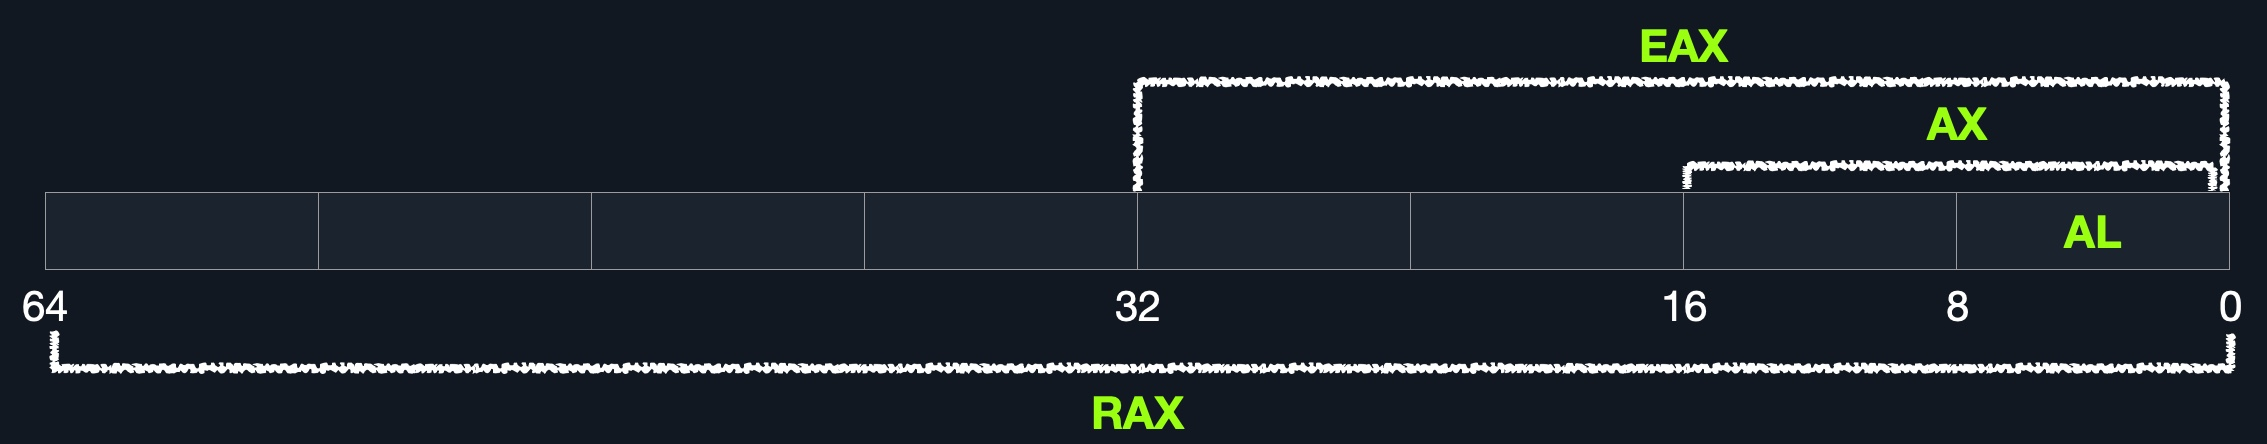
\includegraphics[width=\linewidth]{binary/archi/images/assembly_register_parts.jpg}
  \caption{Registry parts}
  \label{fig:assembly_register_parts}
\end{figure}

\begin{verbatim}
Data/Arguments Registers
    Syscall Number/Return value 	rax 
    Callee Saved 	                rbx 	
    1st arg - Destination operand 	rdi 	
    2nd arg - Source operand  	    rsi 	
    3rd arg 	                    rdx 	
    4th arg - Loop counter 	        rcx 	
    5th arg 	                    r8 	
    6th arg 	                    r9
Pointer Registers
    Base Stack Pointer 	            rbp
    Current/Top Stack Pointer 	    rsp 
    Instruction Pointer 'call only' rip
\end{verbatim}

